\section{Fairness}\label{app:fairness}
\newlength{\fairnessfigurewidth}\setlength{\fairnessfigurewidth}{0.6\columnwidth}

\begin{figure}[htbp]
    \centering
    % \vspace{-10pt}
    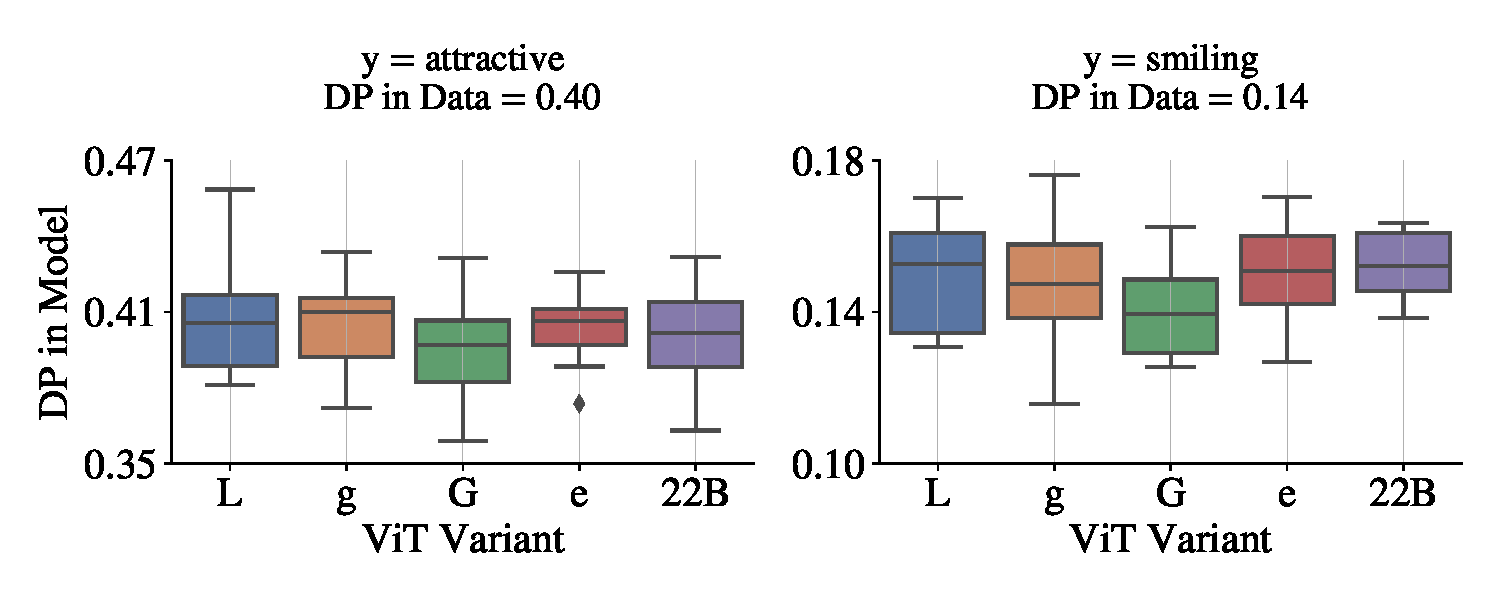
\includegraphics[width=\fairnessfigurewidth]{figs/fairness/bias_original.v3.pdf}
    \vspace{-10pt}
    \caption{DP in the model often reflects DP in the data in the absence of bias mitigation. In this figure, binary sex is the sensitive attribute and linear heads are trained to predict other attributes in CelebA using pretrained features.
    %(e.g. ``L'' is ViT-L). Refer to \cref{sect::fairness} for details.
    }
    \label{fig:fairness:bias_original}
    \vspace{-10pt}
\end{figure}

\begin{figure}[htbp]
    \centering
    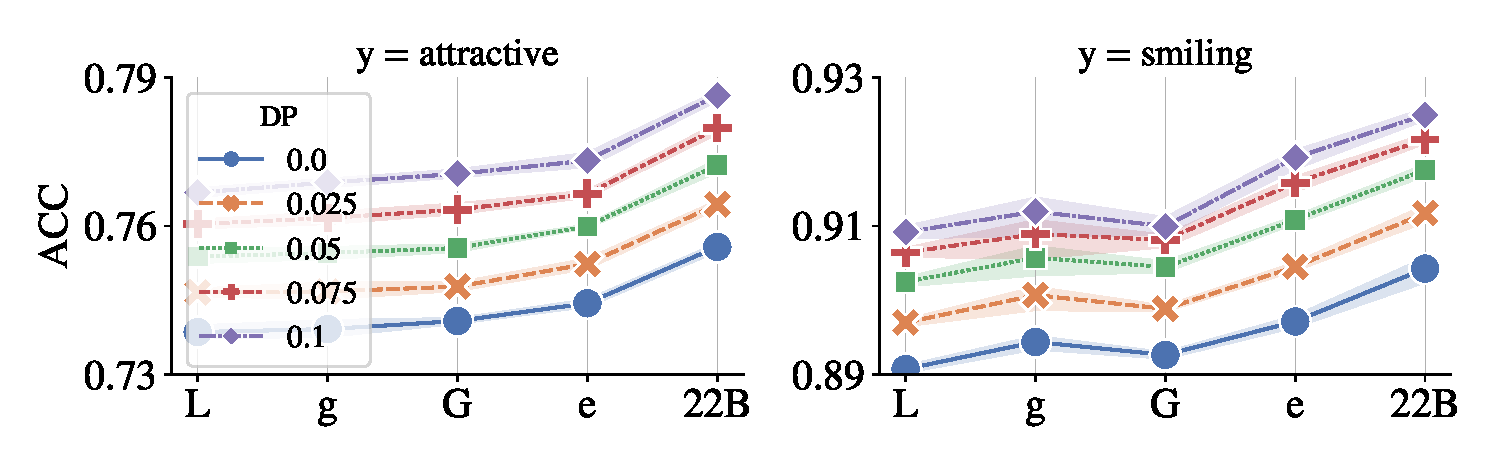
\includegraphics[width=\fairnessfigurewidth]{figs/fairness/perf_acc.v3.pdf}
    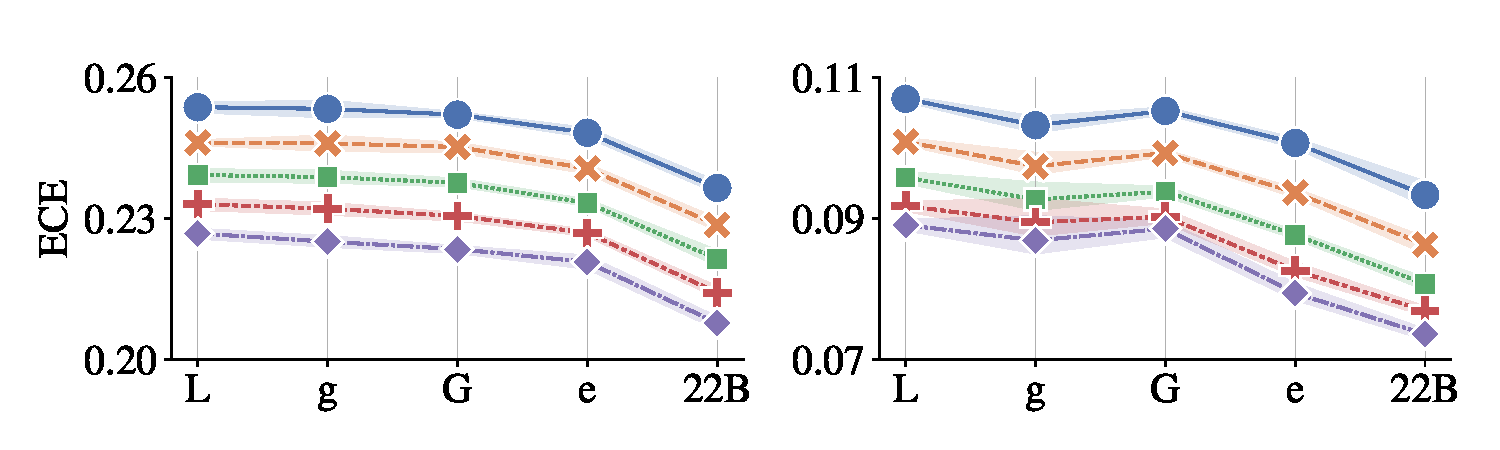
\includegraphics[width=\fairnessfigurewidth]{figs/fairness/perf_ece.v3.pdf}
    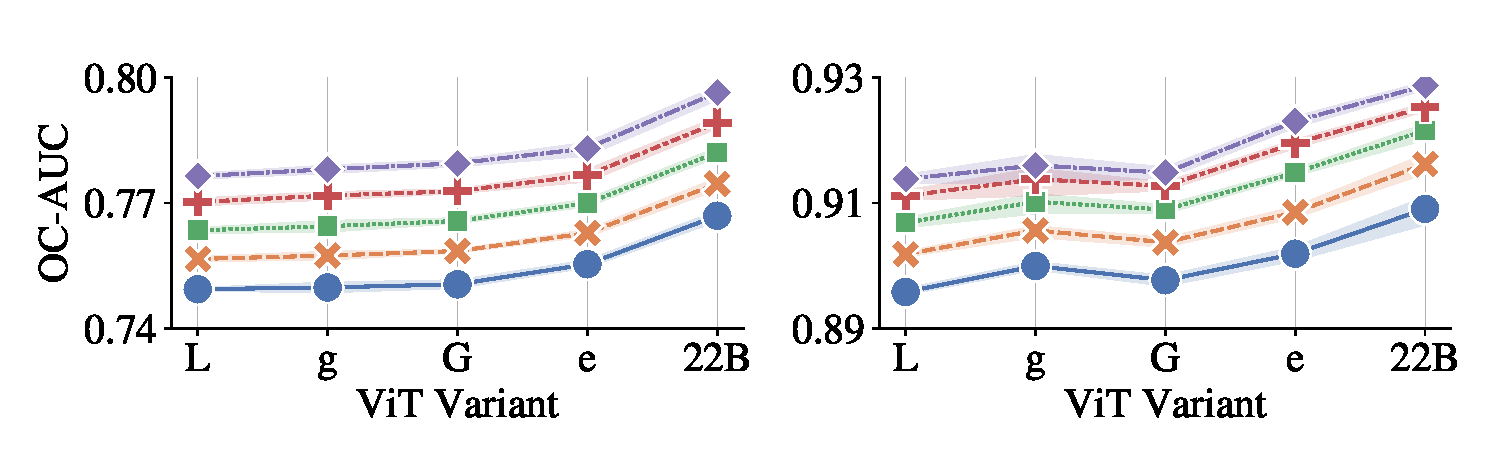
\includegraphics[width=\fairnessfigurewidth]{figs/fairness/perf_ocauc.v3.pdf}\vspace{-1em}
    \caption{Performance, in terms of either accuracy (top),  ECE (middle), or OC-AUC (bottom), is plotted for each ViT variant \emph{after} debiasing the model to meet the prescribed level of bias shown in the legends. Refer to \cref{sect::fairness} for details.}
    \label{fig:fairness:perf}
\end{figure}


\begin{figure}[htbp]
    \centering
    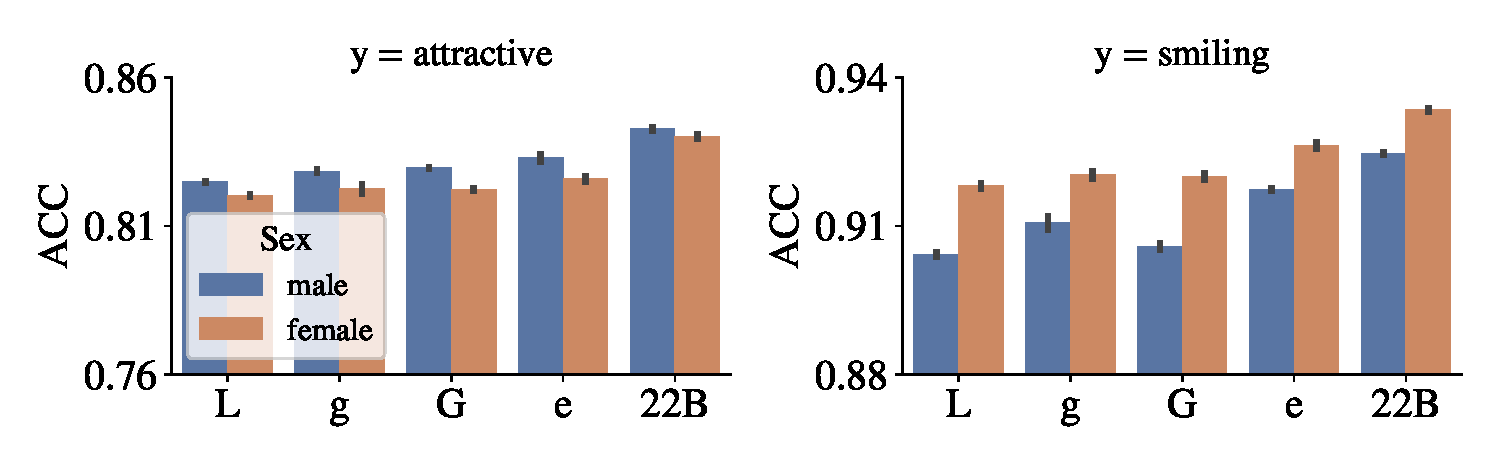
\includegraphics[width=\fairnessfigurewidth]{figs/fairness/all_benefit_acc_1.v3.pdf}
    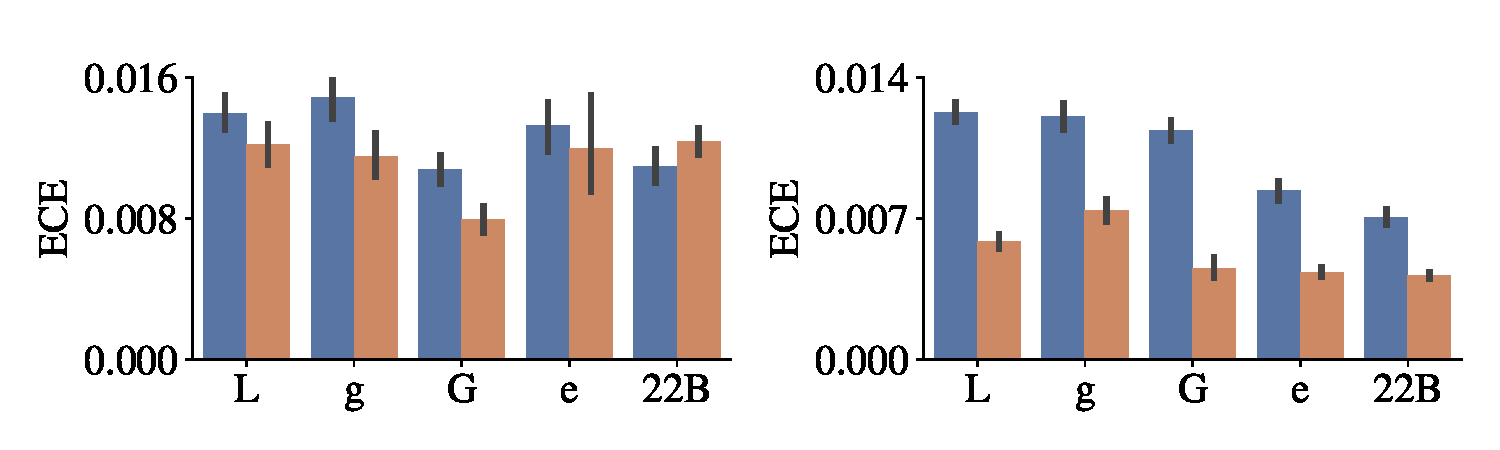
\includegraphics[width=\fairnessfigurewidth]{figs/fairness/all_benefit_ece_1.v3.pdf}
    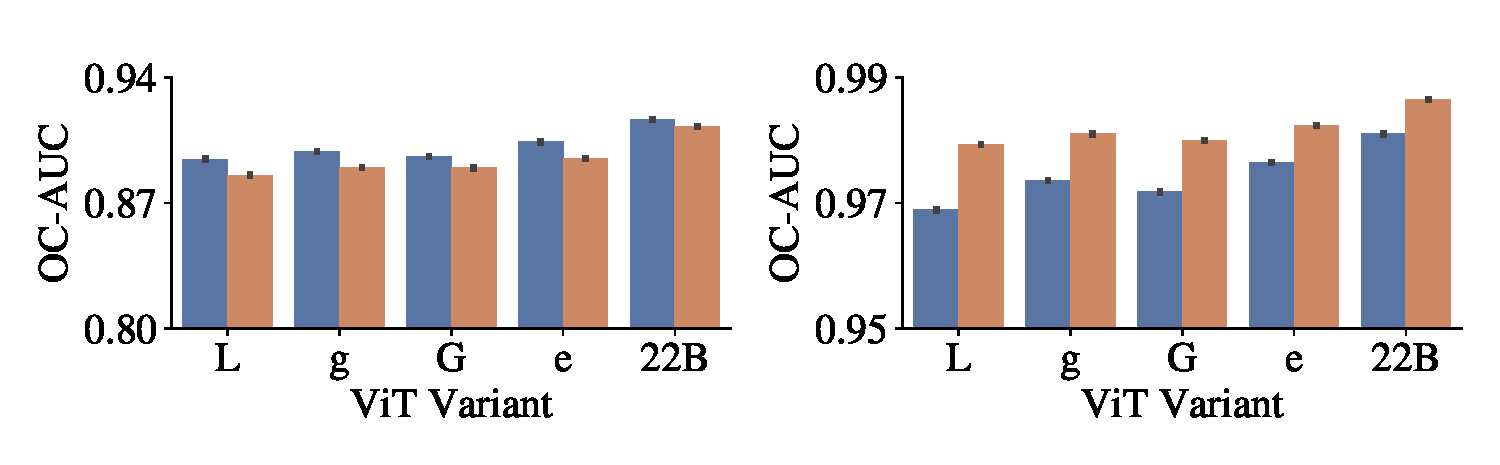
\includegraphics[width=\fairnessfigurewidth]{figs/fairness/all_benefit_ocauc_1.v3.pdf}\vspace{-1em}
    \caption{Performance is plotted for each subgroup in CelebA \emph{prior to} bias mitigation. \chonk offers better performance overall across all three metrics, not just overall, but also within each subgroup separately. Refer to \cref{sect::fairness} for details.}
    \label{fig:fairness:allbenefit}
\end{figure}


\begin{figure}[htbp]
    \centering
    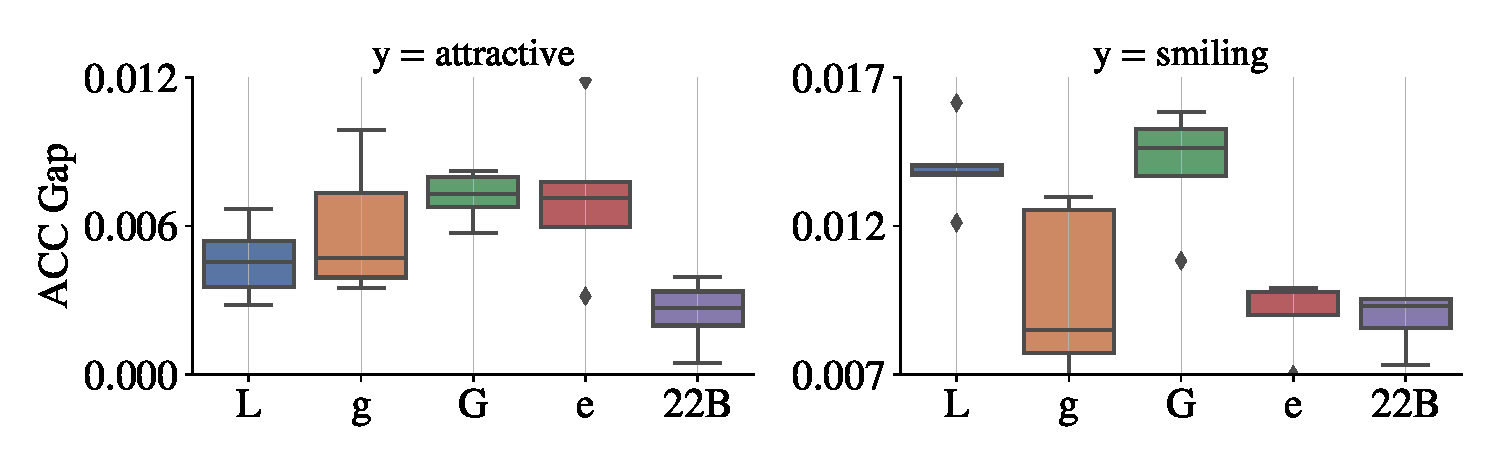
\includegraphics[width=\fairnessfigurewidth]{figs/fairness/parity_acc_1.v3.pdf}
    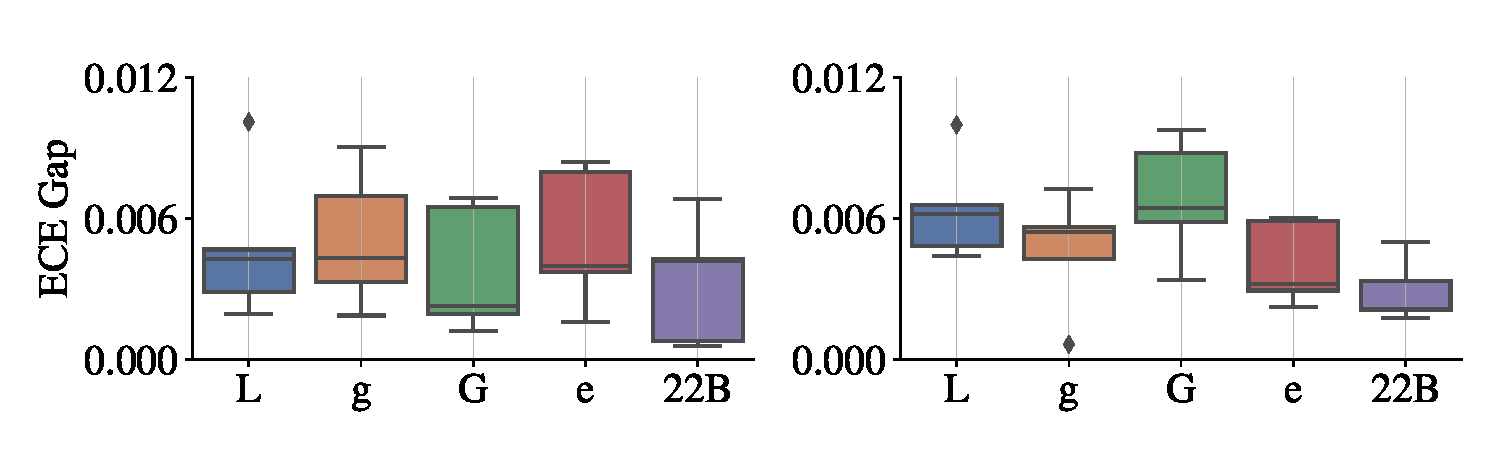
\includegraphics[width=\fairnessfigurewidth]{figs/fairness/parity_ece_1.v3.pdf}
    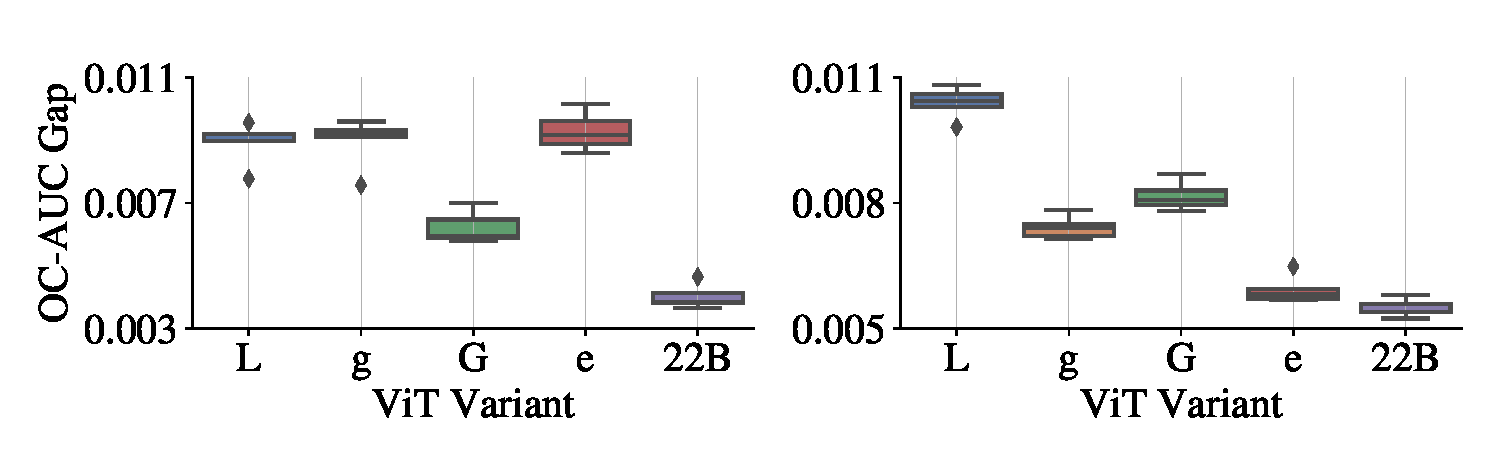
\includegraphics[width=\fairnessfigurewidth]{figs/fairness/parity_ocauc_1.v3.pdf}\vspace{-1em}
    \caption{The $y$-axis is the absolute difference in performance across the two subgroups: females and males. \chonk provides a more equitable performance, compared to earlier/smaller ViT architectures in all three metrics.}
    \label{fig:fairness:parity}
\end{figure}

We report the full experimental results described in \cref{sect::fairness} for all three evaluation (1) classification accuracy (denoted ACC), (2) expected calibration error (ECE)~\citep{naeini2015obtaining,guo2017calibration}, and (3) Oracle Collaborative AUC (OC-AUC)~\citep{kivlichan2021measuring}. 
ECE is used to measure calibration, while OC-AUC computes the four variables: binned true/false positives/negatives, as a function of a linearly spaced set of thresholds and score bins. The full results are presented in \cref{fig:fairness:perf}, \cref{fig:fairness:allbenefit}, and \cref{fig:fairness:parity}.